%!TEX root = bachelor.tex
\chapter{Implementierung}

Zwecks Vereinfachung des Kalibrierungsprozesses wurde ein Assistent in Form einer graphischen Benutzerschnittstelle programmiert. 

Im ersten Schritt des Assistenten wird dabei optional eine intrinsische Kamerakalibrierung durchgeführt (siehe Abbildung \ref{fig:wizard1}). 
\begin{figure}[!htb]
	\centering
	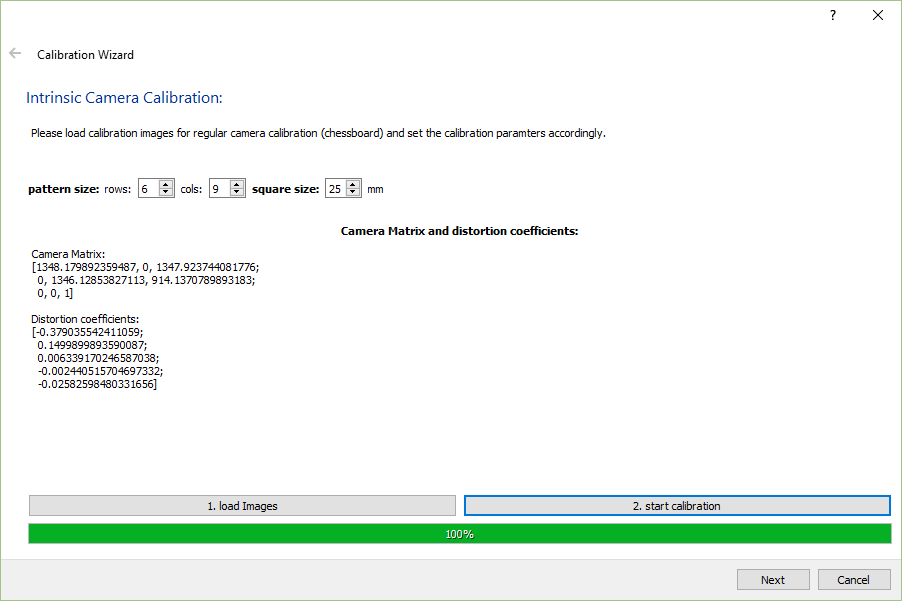
\includegraphics[width=0.9\textwidth]{images/GUI/calibWizard1_1.PNG}
	\caption{Kalibrierungsassistent: intrinsische Kamerakalibrierung}
	\label{fig:wizard1}
\end{figure}

Anschließend wird die eigentliche Kegelkalibrierung ausgeführt. Dabei wird zunächst das Kalibrierungsbild geladen und gegebenenfalls nach einer stattgefundenen intrinsischen Kalibrierung entzerrt. Es werden nun die Sample-Positionen detektiert und der Nutzer hat die Möglichkeit zu überprüfen, ob alle Positionen korrekt detektiert wurden und andernfalls fehlerhafte Punkte zu entfernen und / oder Punkte hinzuzufügen. Im Anschluss werden die Ellipsen und Liniensegmente bestimmt und Punktkorrespondenzen hergestellt (siehe Abbildung \ref{fig:wizard2}).

\begin{figure}[!htb]
	\centering
	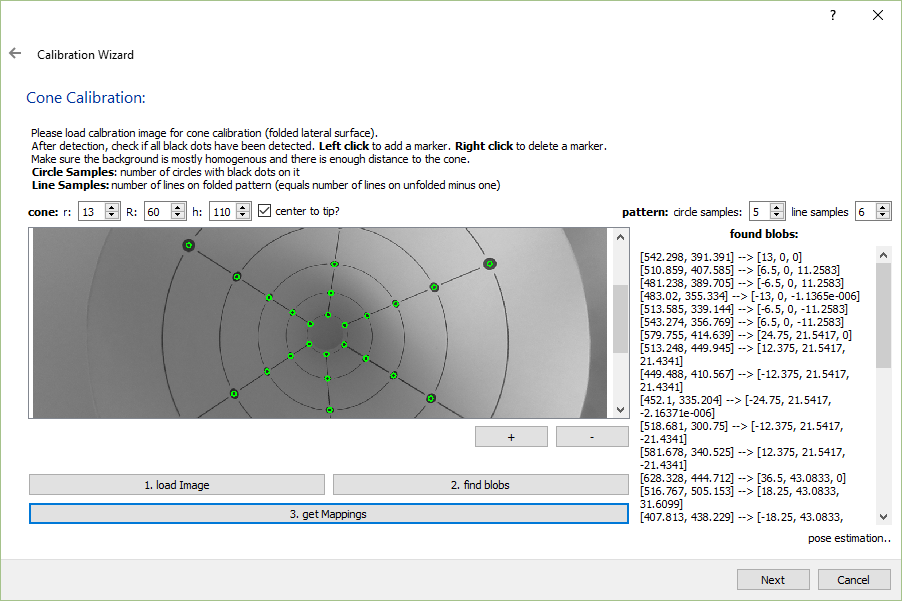
\includegraphics[width=0.9\textwidth]{images/GUI/calibWizard2_1.PNG}
	\caption{Kalibrierungsassistent: Kegelkalibrierung}
	\label{fig:wizard2}
\end{figure}

Im letzten Schritt kann zwischen beiden Entfaltungsverfahren gewählt werden. Anschließend können die Einstellungen in eine XML-Datei exportiert werden, in der, neben der Kamera-Matrix und Verzerrungskoeffizienten, auch die zwei Abbildungsmatrizen des ausgewählten Verfahrens gespeichert werden. 


Die Abbildungsmatrizen sind dabei wie folgt aufgebaut. Als $dst$ bezeichnen wir das entfaltete Bild. $src$ ist das Ursprungsbild.

Bei der Vowärtsentfaltung gilt:
\[
dst(map_x(x,y), map_y(x,y)) = src(x,y),
\]

wobei $map_x$ und $map_y$ die Abbildungsmatrizen sind und die gleiche Größe wie das Ursprungsbild haben. Da wird bei der Entfaltung die Größe des Ergebnisbildes brauchen, und diese bei der Erstellung der Abbildungsmatrizen berechnet haben, sind Breite und Höhe, in $map_x(0,0)$, respektive $map_y(0,0)$, kodiert. Wir verlieren damit die Information $dst(0,0)$ im Ergebnisbild. Dieses Pixel ist aber ohnehin null (siehe zum Beispiel Abbildung \ref{fig:forwardUnfold} in Kapitel \ref{s:unfolding}). 

Bei der Rückwärtsentfaltung gilt:
\[
dst(x,y) = src((map_x(x,y),map_y(x,y)),
\]
wobei $map_x$ und $map_y$ wieder die Abbildungsmatrizen sind und diesmal gleiche Größe wie das entfaltete Bild haben. Eine Kodierung wie bei der Vowärtsentfaltung ist hier also nicht notwendig.
